\documentclass[oneside,monografia]{iftex2020}

% --------------------------------------------------
% Pacotes
% --------------------------------------------------

\usepackage{varwidth}         % Legenda de figuras
\usepackage{fancyvrb}         % Ambiente mono-espaçado
\usepackage{fvextra}          % Melhorias no fancyvrb
\usepackage{textcomp}         % Símbulos extras
\usepackage{tabularx}         % Tabelas

% Ajuste de espaçamento no Verbatim (fancyvrb)
\let\oldverbatim\Verbatim%
\let\oldendverbatim\endVerbatim%
\renewenvironment{Verbatim}%
  {\endgraf\vspace*{-1em}\oldverbatim}%
  {\oldendverbatim\vspace*{-1em}}%

% --------------------------------------------------
% Algoritmos
% --------------------------------------------------
\usepackage[noend]{algpseudocode}
% Comandos para traduzir as instruções do pacote de algoritmos
\algrenewcommand\algorithmicrequire{\textbf{Entrada:}}
\algrenewcommand\algorithmicensure{\textbf{Condição:}}
\algrenewcommand\algorithmicend{\textbf{fim}}
\algrenewcommand\algorithmicif{\textbf{se}}
\algrenewcommand\algorithmicthen{\textbf{então}}
\algrenewcommand\algorithmicelse{\textbf{senão}}
\algrenewcommand\algorithmicfor{\textbf{para}}
\algrenewcommand\algorithmicforall{\textbf{para todo}}
\algrenewcommand\algorithmicdo{\textbf{faça}}
\algrenewcommand\algorithmicwhile{\textbf{enquanto}}
\algrenewcommand\algorithmicrepeat{\textbf{repita}}
\algrenewcommand\algorithmicuntil{\textbf{até que}}
\renewcommand{\Return}{\State \textbf{retorne} }
\let\oldalgorithmic\algorithmic
\let\oldendalgorithmic\endalgorithmic
\renewenvironment{algorithmic}%
  {\hrulefill\vspace*{-0.5em}\oldalgorithmic}%
  {\oldendalgorithmic\vspace*{-1em}\hrulefill}

% --------------------------------------------------
% Comandos personalizados
% --------------------------------------------------
\newcommand{\comando}[1]{\textbf{$\backslash$#1}}
\newcommand{\ifmgtex}[1]{IFMG\TeX}


\addbibresource{referencias.bib}
% Na prática pode ser usado apenas \addbibresource{referencias.bib}
% O comando \addbibresource{referencias.bib} foi usado para mostrar as referências do capítulo de exemplo
\addbibresource[label=bib:exemplo]{referencias_exemplos.bib}

% --------------------------------------------------
% Configurações do Documento
% --------------------------------------------------
\titulo{Classe {\LaTeX} para trabalhos acadêmicos de institutos federais}
\autor{Marcos Roberto Ribeiro}
\local{Bambuí - MG}
\data{15}{dezembro}{2020}

% Instituição
\instituicao{IFMG}{Instituto Federal Minas Gerais}{Instituto Federal de Educação Ciência e Tecnologia de Minas Gerais}
\unidade{\textit{Campus} Bambuí}
\curso{Bacharel}{Bacharelado}{Engenharia de Computação}

% Orientação
\orientador{Nome do Orientador}
% A opção [F] pode ser usada para o feminino
\coorientador[F]{Nome da Coorientadora}
% Caso o coorientador seja de outra instituição
\instituicaocoorientador{Instituição da Coorientadora}

% Membros da banca examinadora (além do orientador e coorientador)
\membrobanca{Fulando de Tal}{Instituição do Fulano de Tal}
\membrobanca{Ciclano de Tal}{Instituição do Ciclano de Tal}

% -------------------------------------------------------
% Elementos Pré-textuais
% -------------------------------------------------------

% --------------------------------------------------
% Resumo e abstract (obrigatórios)
% --------------------------------------------------
\resumo{%
  Este trabalho é um breve modelo de trabalho de conclusão de curso utilizando o ambiente Latex.
  Para a confecção deste modelo foi utilizado o pacote de classes \textit{ABNTex} que segue as normas da Associação Brasileira de Normas Técnicas.
  A elaboração de uma monografia pode ser feita sobrescrevendo o conteúdo deste modelo.
}
\palavraschave{Trabalho de Conclusão de Curso. Latex. Monografia.}


% --------------------------------------------------
% Keywords e abstract
% --------------------------------------------------
\abstract{%
This work is a brief model of course completion work using the Latex environment.
For the preparation of this model was used the package of classes \textit{ABNTex} that follows the norms of the Brazilian Association of Technical Norms.
The elaboration of a monography can be done by overwriting the content of this model.
}
\keywords{Course Completion Work. Latex. Monography.}

% Dedicatória (opcional)
\textodedicatoria{%
À minha esposa e aos meus filhos.

Aos meus pais e à minha irmã.
}

% Agradecimentos (opcional)
\textoagradecimentos{%
Agradeço a todos que contribuíram para a realização deste trabalho.
}

% Epígrafe (opcional)
\textoepigrafe{%
    ``As invenções são, sobretudo, o resultado de um trabalho teimoso.''\\
    (Santos Dumont)
}

% Lista de siglas (opcional)
\listasiglas{%
 \begin{itemize}[]
  \item[ABNT] -- Associação Brasileira de Normas Técnicas
  \item[IFMG] -- Instituto Federal de Educação, Ciência e Tecnologia de Minas Gerais
  \item[SQL] -- \textit{Structured Query Language}
  \item[TCC] -- Trabalho de conclusão de curso
 \end{itemize}
}

% Lista de símbolos (opcional)
\listasimbolos{%
 \begin{itemize}[]
   \item[$\mathbb{X}$] -- Variável X
   \item[$\mathsf{I\!R}$] -- Conjunto dos números reais
 \end{itemize}
}


% Ficha catalográfica (obrigatória)
\ficha{ficha_catalografica}

% --------------------------------------------------
% Folha de aprovação (obrigatória)
% --------------------------------------------------
% Assinaturas e QRCode recortados do documento SEI
\assinaturas{assinaturas}

% -------------------------------------------------------
% Elementos opcionais
% -------------------------------------------------------

% Lista de figuras (opcional)
\listafiguras
% Lista de quadros (opcional)
\listaquadros
% Lista de tabelas (opcional)
\listatabelas
% Lista de algoritmos (opcional)
\listaalgoritmos
% Lista de códigos (opcional)
\listacodigos

\begin{document}

% -------------------------------------------------------
% Gera elementos pré-textuais
% -------------------------------------------------------
\maketitle

% -------------------------------------------------------
% Capítulo: Introdução
% -------------------------------------------------------
\chapter{Introdução} \label{cap:introducao}

Este documento explica brevemente como trabalhar com a classe \textit{Latex} {IF\TeX} para confeccionar trabalhos acadêmicos seguindo as normas da Associação Brasileira de Normas Técnicas (ABNT) e o \textit{Manual de normalização de trabalhos acadêmicos} do IFMG \cite{ifmg:2020:manual}.
O referido manual foi desenvolvido com o intuito de padronizar as trabalhos acadêmicos produzidos na instituição.

A classe {IF\TeX} foi construída com base na classe \textit{abntex2} mantendo as mesmas opções presentes nesta classe, portanto é recomendável que seja consultada a documentação da mesma \cite{araujo:2016:abntex2}.
A classe \textit{abntex2} foi desenvolvida para facilitar a escrita de documentos seguindo as normas da ABNT.
O requisito básico para utilização da classe {IF\TeX} é criar um documento com o comando \comando{documentclass\{iftex2020\}}.
Por padrão, a classe {IF\TeX}, cria um documento frente e verso.
Para documentos somente com anverso, é necessário informar a opção \textbf{onseside} (comando \comando{documentclass[oneside]\{iftex2020\}}).
O tipo de documento deve ser informado como opção também.
Os tipos de documentos possíveis são \textbf{monografia}, \textbf{estagio}, \textbf{dissetacao} e \textbf{tese}.
O tipo de documento padrão é a monografia.
Dessa maneira, para a criação de um relatório de estágio deve ser criado um documento com o comando \comando{documentclass[oneside,estagio]\{iftex2020\}}.


\chapter{Configuração dos elementos pré-textuais}

A configuração de diversas opções e principalmente dos elementos pré-textuais é realizada com comandos específicos inseridos antes do comando \comando{begin\{document\}}. As informações do documento são configuradas através dos comandos:
\begin{description}
\item[\comando{titulo\{T\}}:] Título do trabalho, substitua T pelo título do trabalho;
% --------------------------------------------------
\item[\comando{autor\{N\}}:] Nome do autor do trabalho;
% --------------------------------------------------
\item[\comando{local\{L\}}:] Local do trabalho;
% --------------------------------------------------
\item[\comando{data\{dia\}\{mês (por extenso)\}\{ano\}}:] Configuração da data do documento que aparecerá na folha de aprovação;
% --------------------------------------------------
\item[\comando{instituicao}\{S\}\{N\}\{C\}:] Instituição, onde \textbf{S} é a sigla, \textbf{N} o nome completo e \textbf{C} o nome curto.
Caso não seja informado, a classe adota o comando \comando{instituicao\{IFMG\}\{Instituto Federal Minas Gerais\}\{Instituto Federal de Educação Ciência e Tecnologia de Minas Gerais\}};
\item[\comando{unidade\{U\}}:] Nome da unidade do IF, por exemplo, Campus Bambuí;
% --------------------------------------------------
\item[\comando{curso\{G\}\{T\}\{N\}}:] Dados do curso, são eles grau obtido com o curso(\textbf{G}), tipo do curso (\textbf{T}) e nome do curso (\textbf{N}).
Exemplo: \comando{curso\{Bacharel\}\{Bacharelado\}\{Engenharia de Computação\}\{Bacharel\}};
% --------------------------------------------------
\item[\comando{orientador[G]\{O\}}:] Nome do professor orientador do trabalho.
Caso seja uma orientadora pode ser usado o comando \comando{orientador[F]\{O\}};
% --------------------------------------------------
\item[\comando{coorientador[G]\{C\}}:] Nome do coorientador do trabalho.
Caso seja uma coorientadora pode ser usado um comando análogo a definição de orientadora como \comando{coorientador[F]\{C\}}.
No caso de coorientadores de outras instituições, é preciso usar  comando \comando{instituicaocoorientador\{I\}}, onde \textbf{I} é a instituição do coorientador;
% --------------------------------------------------
\item[Membros da banca avaliadora:] Os membros da banca avaliadora constarão na folha de aprovação juntamente com os nomes do orientador e do coorientador.
A definição dos membros é feita com o comando \comando{membrobanca\{N\}\{I\}}, onde \textbf{N} é o nome do membro e \textbf{I} é sua instituição.
É preciso usar um comando para cada membro;

% --------------------------------------------------
\item[\comando{ficha\{F\}}:] Insere a ficha catalográfica (elemento obrigatório) contida no arquivo \textbf{F}\footnote{A ficha catalográfica é inserida apenas em documentos frente e verso.}.
Entre em contato com a biblioteca para obter a ficha catalográfica em arquivo PDF.
Essa ficha deverá ser inserida no documento após a defesa;
% --------------------------------------------------
\item[\comando{assinaturas\{F\}}:] Insere as assinaturas da folha de aprovação (elemento obrigatório).
Após a defesa, as assinaturas e QRCode devem ser recortados do documento de folha de aprovação no SEI;
% --------------------------------------------------
\item[Dedicatória, Agradecimentos e Epígrafe:] Os elementos pré-textuais opcionais dedicatória, agradecimentos e epígrafe são inseridos com os comandos \comando{textodedicatoria\{T\}}, \comando{textoagradecimentos\{T\}} e \comando{textoepigrafe\{T\}}, respectivamente.

% --------------------------------------------------
\item[Resumo e \textit{Abstract}:] O resumo é incluído com o comando \comando{resumo\{T\}}. Este comando deve ser imediatamente seguido pelo comando \comando{palavraschave\{P\}} para definição das palavras chaves, sendo que P são as palavras chaves iniciando com letras maiúsculas e separadas por pontos. O \textit{Abstract} é configurado de forma análoga com os comandos \comando{abstract\{T\}} e \comando{keywords\{K\}}.
% --------------------------------------------------
\item[\comando{listafiguras}:] Insere a lista de figuras;
% --------------------------------------------------
\item[\comando{listaquadros}:] Insere a lista de quadros;
% --------------------------------------------------
\item[\comando{listatabelas}:] Insere a lista de tabelas;
% --------------------------------------------------
\item[\comando{listaalgoritmos}:] Insere a lista de algoritmos;
% --------------------------------------------------
\item[\comando{listacodigos}:] Insere a lista de códigos;
% --------------------------------------------------
\item[\comando{listasiglas\{L\}}:] Insere a lista de siglas. O parâmetro L é a própria lista de siglas definida em um ambiente \textit{itemize} como mostrado no Código \ref{codigo:lista_siglas};
% --------------------------------------------------
\item[\comando{listasimbolos\{L\}}:] Insere a lista de siglas. O parâmetro L é a definição da lista de símbolos de forma análoga a definição da lista de siglas.
\end{description}

\begin{codigo}[!htb]
\caption{Lista de siglas} \label{codigo:lista_siglas}
\begin{Verbatim}[frame=lines]
\begin{itemize}[]
\item[ABNT] -- Associação Brasileira de Normas Técnicas
\item[IFMG] -- Instituto Federal Minas Gerais
\item[SQL] -- \textit{Structured Query Language}
\item[TCC] -- Trabalho de conclusão de curso
\end{itemize}
\end{Verbatim}
\fonte{Elaborado pelo autor, 2020.}
\end{codigo}


\chapter{Corpos flutuantes}

Corpos flutuantes são elementos não textuais como figuras e tabelas que complementam as informações do texto. Neste capítulo são expostos breves exemplos dos corpos flutuantes disponíveis na classe {IF\TeX}.

Na Seção \ref{secao:figuras} é mostrado como inserir figuras, a Seção \ref{secao:tabelas_e_quadros} explica como incluir tabelas e quadros e a Seção \ref{secao:algoritmos_e_codigos} demostra como trabalhar com algoritmos e códigos fontes.

\section{Figuras}
\label{secao:figuras}

Normalmente, a inserção de figuras é realizada através do comando \comando{begin\{figure\}}.
A Figura \ref{figura:logomarca_if} exibe a logomarca do IF.
É interessante usar o ambiente \texttt{varwidth} em todas as figuras para manter a fonte alinhada a esquerda.
No caso da Figura \ref{figura:logomarca_if}, também foi necessário adicionar uma borda para aumentar o tamanho da figura e manter o alinhamento da fonte.
No caso de figuras de outros autores a citação na fonte deve ser feita com o comando \comando{citefonte\{\}}.

\begin{figure}[!htb] \centering
  \caption{Logomarca do IF} \label{figura:logomarca_if}
  \begin{varwidth}{\linewidth}
    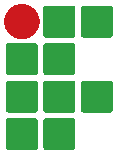
\includegraphics[width=6cm]{figuras/if}
    \fonte{\citefonte{ifmg:2020:manual}.}
  \end{varwidth}
\end{figure}


De acordo com as normas ABNT a lista de figuras é um elemento opcional do documento.
A inclusão de tal lista pode ser feita com o comando \comando{listafiguras} antes do início do documento.

\section{Tabelas e quadros}
\label{secao:tabelas_e_quadros}

A inserção de tabelas e quadros é feita de forma semelhante a inserção de figuras, porém são utilizados os ambientes \textit{table} e \textit{quadro}. A principal diferença entre tabelas e quadros, de acordo com \citet{ifmg:2020:manual}, é que as tabelas são destinadas para informações numéricas e os quadros são mais adequados para informações textuais.

Como exemplos foram inseridas a Tabela \ref{tabela:lista_produtos} que exibe uma de lista de produtos e a Tabela \ref{tabela:populacao_america_sul} que mostra a população dos países da América do Sul. Foi inserido também o Quadro \ref{quadro:editores_texto_livres} com alguns editores que podem ser usados para se trabalhar com Latex para demonstrar a inserção de quadros.

\begin{table}[!htb]
\caption{Lista de produtos} \label{tabela:lista_produtos}
\begin{tabularx}{\textwidth}{X|l|r|r|r} \hline
Produto      & Unidade & Preço (R\$) & Quantidade & Total (R\$) \\ \hline
Arroz        & Kg      & 2,00        & 550        & 1.100,00    \\
Óleo de Soja & L       & 2,50        & 500        & 750,00      \\
Açucar       & Kg      & 3,00        & 100        & 300,00      \\ \hline
\end{tabularx}
\fonte{Elaborado pelo autor, 2020.}
\end{table}

\begin{table}[!htb] \centering
\caption{População dos países da América do Sul} \label{tabela:populacao_america_sul}
\begin{varwidth}{\linewidth}
\begin{tabular}{r|l|r}        \hline
Código  & País            & População   \\ \hline
1       & Brasil          & 191.480.630 \\
2       & Argentina       &  39.934.100 \\
3       & Colômbia        &  46.741.100 \\
4       & Paraguai        &   9.694.200 \\
5       & Uruguai         &   3.350.500 \\
6       & Peru            &  28.221.500 \\
7       & Equador         &  13.481.200 \\
8       & Bolívia         &   9.694.200 \\
9       & Venezuela       &  28.121.700 \\
10      & Chile           &  16.803.000 \\ \hline
\end{tabular}
\fonte{\citefonte{wikipedia:2011:america_sul}.}
\end{varwidth}
\end{table}

\begin{quadro}[!htb] \centering
\caption{Editores de Texto Livres} \label{quadro:editores_texto_livres}
\begin{varwidth}{\linewidth}
\begin{tabular}{|l|l|r|}        \hline
Editor     & Multiplataforma & Específico para Latex \\ \hline
Kwriter    & Sim             & Não                   \\
Texmaker   & Sim             & Sim                   \\
Kile       & Sim             & Sim                   \\
Geany      & Sim             & Não                   \\ \hline
\end{tabular}
\fonte{Elaborado pelo autor, 2020.}
\end{varwidth}
\end{quadro}

A lista de tabelas também é um elemento opcional que pode ser incluída com o comando \comando{listatabelas} antes do início do documento. O mesmo acontece com a lista de quadros que pode ser incluída com o comando \comando{listaquadros}.

\section{Algoritmos e códigos} \label{secao:algoritmos_e_codigos}

Além dos corpos flutuantes convencionais para inserir figuras (\comando{begin\{figure\}}) e tabelas (\comando{begin\{figure\}}), a classe {IF\TeX} possui mais dois tipos de corpos flutuantes um para algoritmos (\comando{begin\{algoritmo\}}) e outro para códigos (\comando{begin\{codigo\}}). Como exemplo temos o Algoritmo \ref{algoritmo:mdc} que calcula o máximo divisor comum entre dois números e os Códigos \ref{codigo:notas_alunos} e \ref{codigo:metodo_leitura} que são uma consulta na \textit{Structured Query Language (SQL)} e um método em Java que recebe um texto digitado pelo usuário, respectivamente.

\begin{algoritmo}[!htb]
\caption{Algoritmo para cálculo de máximo divisor comum MDC($n_1$,$n_2$)} \label{algoritmo:mdc}
\begin{algorithmic}[1]
 \Require Dois números inteiros ($n_1, n_2$)
 \If{$n_2 > n_1$} \Comment{Garante que o maior número seja $n_1$}
   \State troca valores de $n_1$ e $n_2$
 \EndIf
 \Repeat
   \State $r \leftarrow$ resto da divisão de $n_1$ por $n_2$
   \State $n_1 \leftarrow n_2$
   \State $n_2 \leftarrow r$
 \Until{$r > 0$}
 \Return $n_1$
\end{algorithmic}
\fonte{Elaborado pelo autor, 2020.}
\end{algoritmo}

\begin{codigo}[!htb]
\caption{Consulta SQL} \label{codigo:notas_alunos}
\begin{Verbatim}[frame=lines]
SELECT a.nome_aluno AS aluno,
       d.nome_disciplina AS disciplina,
       m.nota AS nota
FROM aluno AS a,
     disciplina AS d,
     matriculado AS m
WHERE a.id_aluno = m.id_aluno
  AND d.id_disciplina = m.id_disciplina
ORDER BY a.nome_aluno, d.nome_disciplina;
\end{Verbatim}
\fonte{Elaborado pelo autor, 2020.}
\end{codigo}

\begin{codigo}[!htb]
\caption{Sub-rotina para obter uma entrada do usuário} \label{codigo:metodo_leitura}
\begin{Verbatim}[frame=lines]
public static String Leitura(){
    BufferedReader reader =
        new BufferedReader(new InputStreamReader(System.in));
    try {
        return reader.readLine(); // Lê uma linha pelo teclado
    } catch (IOException e) {
        e.printStackTrace();
        return "";
    }
}
\end{Verbatim}
\fonte{Elaborado pelo autor, 2020.}
\end{codigo}

Existem diversos outros pacotes disponíveis para escrever algoritmos e códigos. Nos exemplos anteriormente foram utilizados o pacote \textit{algpseudocode} e \textit{fancyvrb}. O pacote \textit{algpseudocode} é usado para escrever algoritmos em alto nível \cite{janos:2005:algpseudocode}. Já o pacote \textit{fancyvrb} serve para escrever códigos mono-espaçados \cite{zandt:2010:fancyvrb}.
Caso sejam utilizados os ambientes de algoritmo e código, podem ser incluídos os comandos \comando{listaalgoritmos} e \comando{listacodigos} antes do \comando{begin\{document\}} para que a lista de algoritmos e a lista de código sejam criadas.
Existem também diversos outros pacotes para formatação de algoritmos e códigos que podem ser usados como o \textit{minted} com suporte a diversas linguagens de programação \cite{poore:2016:minted}.


\chapter{Ambientes matemáticos}

A classe {IF\TeX} provê os seguintes ambientes matemáticos:
\begin{itemize}
 \item Teoremas (\comando{begin\{teorema\}[\ ]} ... \comando{begin\{teorema\}});
 \item Proposição (\comando{begin\{proposicao\}[\ ]} ... \comando{begin\{proposicao\}});
 \item Lema (\comando{begin\{lema\}[\ ]} ... \comando{begin\{lema\}});
 \item Corolário (\comando{begin\{corolario\}[\ ]} ... \comando{begin\{corolario\}});
 \item Exemplo (\comando{begin\{exemplo\}[\ ]} ... \comando{begin\{exemplo\}});
 \item Observação (\comando{begin\{observacao\}[\ ]} ... \comando{begin\{observacao\}});
 \item Definição (\comando{begin\{definicao\}[\ ]} ... \comando{begin\{definicao\}});
 \item demonstracao (\comando{begin\{demonstracao\}[\ ]} ... \comando{begin\{demonstracao\}}).
\end{itemize}

Abaixo temos um exemplo de proposição com sua demonstração:
\begin{proposicao}
 Sejam $a$ e $b$ reais, tais que $0<a<b$. Então $a^2<b^2$.
\end{proposicao}
\begin{demonstracao}
 Pela hipótese concluímos que $(b+a)>0$ e $(b-a)>0$.

Como $b^2-a^2=(b+a)(b-a)$ concluímos que $b^2-a^2>0$, ou seja, $a^2<b^2$.
\end{demonstracao}

Neste documento tratamos brevemente apenas dos ambientes mencionados anteriormente. Contudo, para escrever expressões matemáticas complexas é preciso estudar uma documentações mais específicas\footnote{\url{https://en.wikibooks.org/wiki/LaTeX/Mathematics}}\footnote{\url{https://en.wikibooks.org/wiki/LaTeX/Advanced_Mathematics}}.
Alguns dos ambientes matemáticos da classe {IF\TeX} podem ser usados também para outras finalidades como exemplos e definições.


\chapter{Ferramentas úteis} \label{capitulo:ferramentas_uteis}

Existem diversas ferramentas para se trabalhar com Latex. Duas ferramentas que merecem destaque são o editor \textit{Texmaker} exibido na Figura \ref{figura:texmaker} e o gerenciador de referências \textit{JabRef} mostrado na Figura \ref{figura:jabref}. Ambas ferramentas são livres e multiplataforma.

\begin{figure}[!htb]
 \caption{Tela do Texmaker} \label{figura:texmaker}
 \begin{varwidth}{\linewidth}
  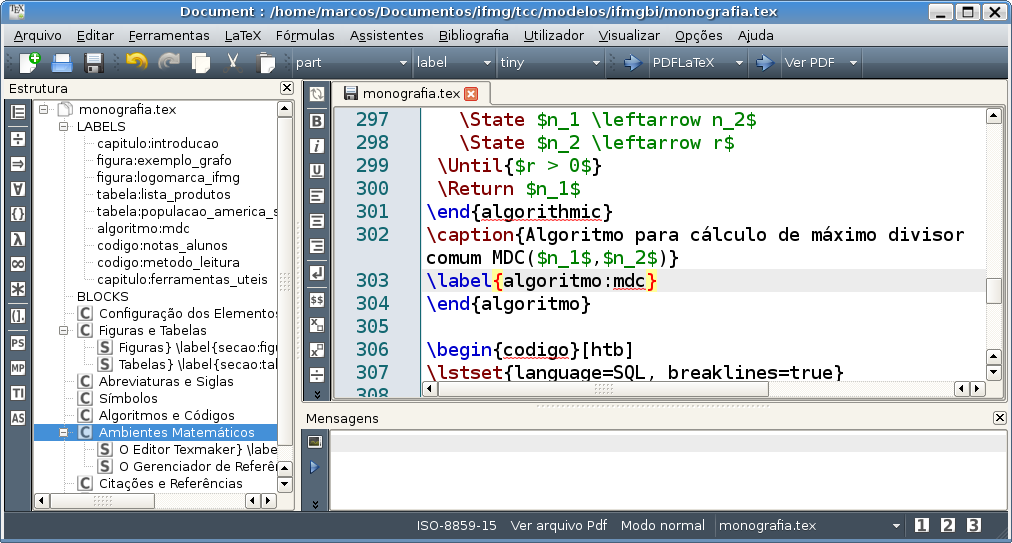
\includegraphics[width=\textwidth]{figuras/texmaker}
 \end{varwidth}
 \fonte{Elaborado pelo autor, 2020.}
\end{figure}

\begin{figure}[!htb]
 \caption{Tela do JabRef} \label{figura:jabref}
 \begin{varwidth}{\linewidth}
  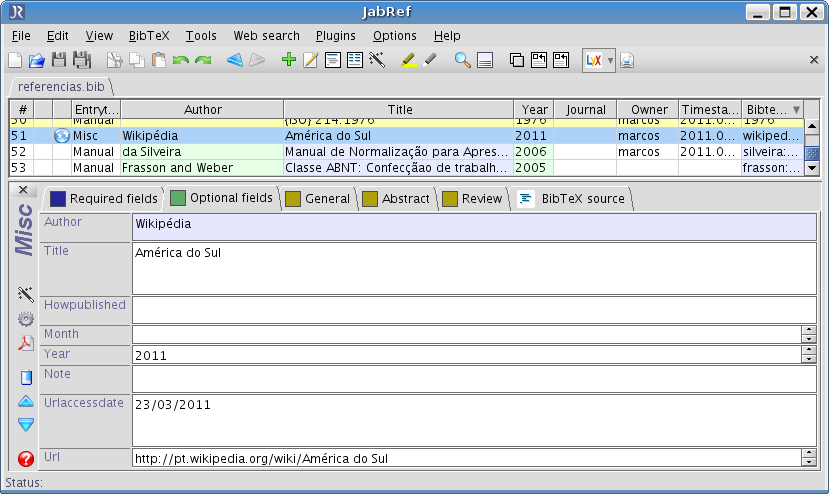
\includegraphics[width=\textwidth]{figuras/jabref}
 \end{varwidth}
 \fonte{Elaborado pelo autor, 2020.}
\end{figure}

O Texmaker pode ser obitido em \url{http://www.xm1math.net/texmaker} e o JabRef pode ser obtido em \url{http://www.jabref.org/}. É importante ressaltar que o Texmaker é apenas um editor, para compilar os documentos é necessário um ambiente Latex instalado. Os ambientes Latex mais populares são o Texlive (\url{http://www.tug.org/texlive}) e o MiKTex (\url{http://miktex.org}).


\chapter{Citações}

Em documentos acadêmicos podem existir citações diretas e citações indiretas. As citações indiretas são feitas quando se reescreve uma referência consultada. Nas citações indiretas há duas formatações possíveis dependendo de como ocorre a citação no texto. Quando o autor é mencionado explicitamente na sentença deve ser usado o comando \comando{citet\{\}}, nas demais situações é usado o comando \comando{cite\{\}}. A Figura \ref{figura:citacao_indireta_explicita} mostra um exemplo com o comando \comando{citet\{\}}.

% --------------------------------------------------

\begin{figure}[!htb]
\caption{Exemplo de citação indireta explícita} \label{figura:citacao_indireta_explicita}

\hrulefill\vspace*{-1em}

\begin{verbatim}
Segundo \citet{ifmg:2020:manual}, o trabalho de conclusão de curso
deve seguir as normas da ABNT.
\end{verbatim}

\vspace*{-1.5em}\hrulefill

Segundo \citet{ifmg:2020:manual}, o trabalho de conclusão de curso deve seguir as normas da ABNT.

\vspace*{-0.5em}\hrulefill
\fonte{Elaborado pelo autor, 2020.}
\end{figure}

% --------------------------------------------------

Para especificar a página consultada na referência é preciso acrescentá-la entre colchetes com os comandos \comando{cite[página]\{\}} ou \comando{citet[página]\{\}}. Na Figura \ref{figura:citacao_indireta_pagina} é mostrado um exemplo de citação com página específica.

% --------------------------------------------------

\begin{figure}[!htb]
\caption{Exemplo de citação indireta não explícita} \label{figura:citacao_indireta_pagina}
\hrulefill\vspace*{-1em}

\begin{verbatim}
A folha de aprovação é um elemento obrigatório no trabalho de conclusão
de curso \cite[p.~22]{ifmg:2020:manual}.
\end{verbatim}

\vspace*{-1.5em}\hrulefill

A folha de aprovação é um elemento obrigatório no trabalho de conclusão de curso \cite[p.~22]{ifmg:2020:manual}.

\vspace*{-0.5em}\hrulefill
\fonte{Elaborado pelo autor, 2020.}
\end{figure}

% --------------------------------------------------

As citações diretas acontecem quando o texto de uma referência é transcrito literalmente. As citações diretas são curtas (até três linhas) são inseridas no texto entre aspas duplas. Como no exemplo mostrado na Figura \ref{figura:citacao_direta_curta}.

% --------------------------------------------------

\begin{figure}[!htb]
\caption{Exemplo de citação direta curta} \label{figura:citacao_direta_curta}
\hrulefill\vspace*{-1em}

\begin{verbatim}
``A tabela deve ser colocada em posição vertical, para facilitar a
leitura dos dados'' \cite[p.~26]{ifmg:2020:manual}.
\end{verbatim}

\vspace*{-1.5em}\hrulefill

``A tabela deve ser colocada em posição vertical, para facilitar a leitura dos dados'' \cite[p.~25]{ifmg:2020:manual}.

\vspace*{-0.5em}\hrulefill
\fonte{Elaborado pelo autor, 2020.}
\end{figure}

% --------------------------------------------------

As citações longas (com mais de 3 linhas) podem ser inseridas com o ambiente \comando{begin\{citacao\}} como mostra a Figura \ref{figura:citacao_direta_longa}.

% --------------------------------------------------

\begin{figure}[!htb]
\caption{Exemplo de citação direta longa} \label{figura:citacao_direta_longa}
\hrulefill\vspace*{-1em}

\begin{verbatim}
\begin{citacao}
A tabela deve ser colocada em posição vertical, para facilitar a
leitura dos dados.
No caso em que isso seja impossível, deve ser colocada em posição
horizontal, com o título voltado para a margem esquerda da folha.
Fontes e notas devem aparecer na parte inferior da
tabela em tamanho 11 \cite[p.~25]{ifmg:2020:manual}.
\end{citacao}
\end{verbatim}

\vspace*{-1.5em}\hrulefill

\begin{citacao}
A tabela deve ser colocada em posição vertical, para facilitar a leitura dos dados. No
caso em que isso seja impossível, deve ser colocada em posição horizontal, com o título
voltado para a margem esquerda da folha. Fontes e notas devem aparecer na parte inferior da
tabela em tamanho 11 \cite[p.~25]{ifmg:2020:manual}.
\end{citacao}

\vspace*{-0.5em}\hrulefill
\fonte{Elaborado pelo autor, 2020.}
\end{figure}


\chapter{Modelos de referências}

Este capítulo apresenta alguns modelos de referências \cite{ifmg:2020:manual}.

\section{Livro e/ou Folheto}

Os elementos essenciais são: autor(es), título, subtítulo (se houver), edição, local, editora e data de publicação.
Alguns exemplos:

\vspace*{1em}

\begin{Verbatim}[frame=single]
@book{chiavenato:2014,
  author    = {Idalberto Chiavenato},
  title     = {Administração},
  subtitle  = {teoria, processo e prática},
  edition   = {5},
  address   = {Barueri},
  publisher = {Manole},
  year      = {2014},
  note      = {\textit{E-book}.},
}
\end{Verbatim}

\noindent
\fullcite{chiavenato:2014}.

\vspace*{1em}

\begin{Verbatim}[frame=single]
@book{fazio:2011,
  author    = {Fazio, Michael W. and
               Moffett, Marian and
               Wodehouse, Lawrence},
  title     = {A história da arquitetura mundial},
  edition   = {3},
  address   = {Porto Alegre},
  publisher = {AMGH},
  year      = {2011},
}
\end{Verbatim}

\noindent
\fullcite{fazio:2011}.

\section{Trabalho acadêmico}

São considerados trabalhos acadêmicos: trabalho de conclusão de curso, dissertações, teses e outros trabalhos acadêmicos considerados no todo.
Os itens essenciais são: autor(es), título, subtítulo (se houver), ano de depósito, tipo do trabalho (tese, dissertação, trabalho de conclusão de curso e outros), grau (graduação, especialização, mestrado ou doutorado) seguido do curso entre parênteses, vinculação acadêmica e data de apresentação ou defesa.
Alguns exemplos:

\vspace*{1em}

\begin{Verbatim}[frame=single]
@thesis{oliveira:2016:app_fruta,
  title       = {Desenvolvimento de um aplicativo em plataforma {Android}
                 para auxílio no ensino de {Fruticultura}},
  author      = {Oliveira, Bruno Alberto Soares and
                 Silva, Gabriel da},
  type        = {Relatório Final de Projeto de Iniciação Científica
                 (Graduação em Engenharia de Computação)},
  institution = {Instituto Federal de Educação, Ciência e Tecnologia de
                 Minas Gerais (IFMG)},
  location    = {Bambuí},
  eventyear   = {2016},
  year        = {2016},
}
\end{Verbatim}

\noindent
\fullcite{oliveira:2016:app_fruta}.

\vspace*{1em}

\begin{Verbatim}[frame=single]
@thesis{vieira:2020:cpresql,
  title       = {Novo modelo de hierarquia de preferências em consultas
                 com preferências condicionais},
  author      = {Vieira, Lucas Mariano},
  type        = {Trabalho de Conclusão de Curso (Graduação em Engenharia
                 de Computação)},
  institution = {Instituto Federal de Educação, Ciência e Tecnologia de
                 Minas Gerais (IFMG)},
  location    = {Bambuí},
  eventyear   = {2020},
  year        = {2020},
}
\end{Verbatim}

\noindent
\fullcite{vieira:2020:cpresql}.

\vspace*{1em}

\begin{Verbatim}[frame=single]
@thesis{nascimento:2001,
  author      = {Suzy Regina Nascimento},
  title       = {Oscilações no desempenho de motoristas profissionais,
                 motoristas pluriacidentados e não-motoristas em tarefas
                 de atenção mantida},
  type        = {Dissertação (Mestrado em Psicologia)},
  institution = {Instituto de Psicologia, Universidade de São Paulo
                 (USP)},
  location    = {São Paulo},
  eventyear   = {2001},
  year        = {2001},
}
\end{Verbatim}

\noindent
\fullcite{nascimento:2001}.

\vspace*{1em}

\begin{Verbatim}[frame=single]
@thesis{ribeiro:2018,
  author      = {Marcos Roberto Ribeiro},
  title       = {{StreamPref}},
  subtitle    = {Uma linguagem de consulta para dados em fluxo com
                 suporte a preferências},
  type        = {Tese (Doutorado em Ciência da Computação)},
  institution = {Faculdade de Computação, Universidade Federal de
                 Uberlândia (UFU)},
  location    = {Uberlândia},
  eventyear   = {2018},
  year        = {2018},
}
\end{Verbatim}

\noindent
\fullcite{ribeiro:2018}.

\section{Parte de trabalho}

Inclui capítulo, volume, fragmento e outras partes de uma obra, com autor(es) e/ou título próprios.
Os elementos essenciais são: autor(es), título da parte, seguidos da expressão ``In:'', e da referência completa da monografia no todo. No final da referência, deve-se informar a descrição física da parte.
Exemplo:

\vspace*{1em}

\begin{Verbatim}[frame=single]
@incollection{martins:2015,
  author     = {José Rodolfo S. Martins},
  title      = {Obras de macrodrenagem},
  pages      = {167--240},
  booktitle  = {Drenagem urbana},
  editor     = {TUCCI, Carlos E. M. Tucci and
                Rubem La Laina P. Porto and
                Mário T. Barros},
  editortype = {org.},
  publisher  = {ABRH},
  location   = {Porto Alegre},
  year       = {2015},
}
\end{Verbatim}

\noindent
\fullcite{martins:2015}.

\section{Periódicos}

Nas referências a periódicos como todo, os elementos essenciais são: título, subtítulo (se houver), local de publicação, editora, datas de início e de encerramento da publicação (se houver), e ISSN (se houver).
Exemplo:

\vspace*{1em}

\begin{Verbatim}[frame=single]
@article{techne:1993,
  title     = {TÉCHNE},
  subtitle  = {revista de tecnologia da construção},
  year      = {1993-},
  location  = {São Paulo},
  publisher = {Pini},
  issn      = {0104-1053},
}
\end{Verbatim}

\noindent
\fullcite{techne:1993}.

\vspace*{1em}

Para os artigos de periódico, os elementos essenciais são: autor (es), título do artigo ou da matéria, subtítulo (se houver), título do periódico, subtítulo (se houver), local de publicação, numeração do volume e/ou ano, número e/ou edição, tomo (se houver), páginas inicial e final, e data ou período de publicação.
Exemplo:

\vspace*{1em}

\begin{Verbatim}[frame=single]
@article{lelis:2004,
  author    = {Lelis, V. G. and
               Costa, E. D. and
               Ramos, L. P. and
               Alvarenga, L. M. and
               Minim, V. P. R. M.},
  title      = {Aceitabilidade sensorial de doce de leite de diferentes
                sabores},
  journal    = {Revista do Instituto de Laticínios Cândido Tostes},
  volume     = {59},
  number     = {339},
  pages      = {324-327},
  month      = {jan},
  year       = {2004},
  location   = {Juiz de Fora},
}
\end{Verbatim}

\noindent
\fullcite{lelis:2004}.

\vspace*{1em}

No caso de artigo ou matéria de jornal, os elementos essenciais são: autor(es), título do artigo, subtítulo (se houver), título do jornal, subtítulo de jornal (se houver), local de publicação, numeração do ano e/ou volume, número, data de publicação, seção, caderno ou parte do jornal e a paginação correspondente.
Exemplo:

\vspace*{1em}

\begin{Verbatim}[frame=single]
@article{naves:1999,
  author       = {P. Naves},
  title        = {Lagos andinos dão banho de beleza},
  journaltitle = {Folha de S. Paulo},
  location     = {São Paulo},
  date         = {1999-06-28},
  note         = {Folha Turismo, Caderno 8, p. 13},
}
\end{Verbatim}

\noindent
\fullcite{naves:1999}.

\section{Evento}

Um evento é o resultado de trabalhos publicados em congressos, seminários, simpósios, encontros, semanas, etc.

Nas referências a um evento como todo, os elementos essenciais são: nome do evento, numeração (se houver), ano e local (cidade) de realização, título do documento, seguidos dos dados de local, editora e data da publicação.
Exemplo:

\vspace*{1em}


\begin{Verbatim}[frame=single]
@proceedings{labid,
  eventtitle = {Congresso Latino-Americano de Biblioteconomia e
                Documentação},
  number     = {1},
  venue      = {Salvador},
  eventyear  = {1980},
  title      = {Anais [...]},
  publisher  = {FEBAB},
  address    = {Salvador},
  year       = {1980},
  pagetotal  = {350},
}
\end{Verbatim}

\noindent
\fullcite{labid}.

\vspace*{1em}

Para trabalhos publicados em eventos, Os elementos essenciais são: autor, título do trabalho, seguidos da expressão In: nome do evento, numeração do evento (se houver), ano e local (cidade) de realização, título do documento, local, editora e data da publicação e páginas inicial e final da parte referenciada.
Exemplo:

\vspace*{1em}

\begin{Verbatim}[frame=single]
@inproceedings{brayner:1994,
  author     = {Brayner, A. R. A. and
                Medeiros, C. B.},
  title      = {Incorporação do tempo em SGBD orientado a objetos},
  eventtitle = {Simpósio Brasileiro de Banco de Dados (SBBD)},
  number     = {IX},
  venue      = {São Paulo},
  eventyear  = {1994},
  booktitle  = {Anais [...]},
  publisher  = {USP},
  address    = {São Paulo},
  year       = {1994},
  pages      = {16--29},
}
\end{Verbatim}

\noindent
\fullcite{brayner:1994}.

\section{Patente}

Os elementos essenciais de patentes são: inventor (autor), título, nomes do depositante ou titular e do procurador (se houver), número da patente, data de depósito e data de concessão da patente (se houver).
Exemplo:

\vspace*{1em}

\begin{Verbatim}[frame=single]
@patent{bertazzoli:2006,
  author     = {Bertazzoli, Rodnei and
                Silva, João and
                Mendes, José and
                Carvalho, Maria},
  title      = {Eletrodos de difusão gasosa modifi cados com
                catalisadores redox, processo e reator eletroquímico de
                síntese de peróxido de hidrogênio utilizando os mesmos},
  titleaddon = {Depositante: Universidade Estadual de Campinas.
                Procurador: Maria Cristina Valim Lourenço Gomes},
  number     = {BR n. PI0600460-1A},
  note       = {Depósito: 27 jan. 2006. Concessão: 25 mar. 2008},
}
\end{Verbatim}

\noindent
\fullcite{bertazzoli:2006}.

\section{Legislação}

Referências a legislações incluem Constituição, Decreto, Decreto-Lei, Emenda Constitucional, Emenda à Lei Orgânica, Lei Complementar, Lei Delegada, Lei Ordinária e Medida Provisória, entre outros.
Os elementos essenciais são: jurisdição, ou cabeçalho da entidade, em letras maiúsculas; epígrafe e ementa transcrita conforme publicada; dados da publicação.

Quando necessário, acrescentam-se à referência os elementos complementares para melhor identificar o documento, como: retificações, alterações, revogações, projetos de origem,
autoria do projeto, dados referentes ao controle de constitucionalidade, vigência, eficácia, consolidação ou atualização.
Em epígrafes e ementas demasiadamente longas, pode-se suprimir parte do texto, desde que não seja alterado o sentido. A supressão deve ser indicada por reticências, entre colchete.
Alguns exemplos:

\vspace*{1em}

\begin{Verbatim}[frame=single]
@legislation{brasil2002,
  author     = {{Brasil}},
  nameaddon  = {[Constituição (1988)]},
  title      = {Constituição da República Federativa do Brasil},
  titleaddon = {Organizado por Cláudio Brandão de Oliveira},
  location   = {Rio de Janeiro},
  publisher  = {Roma Victor},
  year       = {2002},
}
\end{Verbatim}

\noindent
\fullcite{brasil2002}.

\vspace*{1em}

\begin{Verbatim}[frame=single]
@legislation{curitiba2007,
  author     = {{Curitiba}},
  title      = {Lei n. 12.092, de 21 de dezembro de 2006},
  titleaddon = {Estima a receita e fixa a despesa do município de
                curitiba para o exercício financeiro de 2007},
  location   = {Curitiba},
  publisher  = {Câmara Municipal},
  year       = {[2007]},
  url        = {http://dominio.cmc.pr.gov.br/contlei.nsf/l12092-2006},
  urldate    = {2007-03-22},
}
\end{Verbatim}

\noindent
\fullcite{curitiba2007}.

\section{Documento cartográfico}

Documentos cartográficos incluem atlas, mapa, globo, fotografia aérea, entre outros.
Elementos essenciais: autor(es), título, subtítulo (se houver), local, editora, data de publicação, descrição física e escala (se houver). Quando necessário, acrescentam-se elementos complementares à referência para melhor identificar o documento.
Exemplo:

\vspace*{1em}

\begin{Verbatim}[frame=single]
@image{brasil1979,
  author    = {{Brasil}},
  nameaddon = {Ministério da Marinha},
  title     = {Brasil - costa leste},
  subtitle  = {do Rio Itatiti a Ilhéus},
  edition   = {3},
  location  = {Rio de Janeiro},
  year      = {1979},
  note      = {Carta náutica, N. 1.100. Escala natural 1: 308.541 na lat.
               13° 23,50'.},
}
\end{Verbatim}

\noindent
\fullcite{brasil1979}.


\section{Meio eletrônico}

Para informações de acesso exclusivo por meio eletrônico, os elementos essenciais: autor(es), título da informação ou serviço ou produto, versão ou edição (se houver), local, data e descrição física do meio eletrônico. Informações sobre o endereço eletrônico, precedido da expressão ``Disponível em:'' e a data de acesso ao documento, precedida da expressão ``Acesso em:''.

Os demais tipos referências em meio eletrônico devem obedecer aos padrões já especificados, acrescidas das informações relativas à descrição física do meio eletrônico e a data de acesso.


Alguns exemplos de referências em meios eletrônicos:

\vspace*{1em}

\begin{Verbatim}[frame=single]
@online{nourau,
  title      = {NOU-Rau},
  titleaddon = {software livre},
  version    = {Beta 2},
  location   = {Campinas},
  publisher  = {UNICAMP},
  year       = {2002},
  url        = {www.rau-tu.unicamp.br/nou-rau},
  urldate    = {2002-04-23},
}
\end{Verbatim}

\noindent
\fullcite{nourau}.

\vspace*{1em}

\begin{Verbatim}[frame=single]
@book{galt:2017,
  author    = {Christopher Galt},
  title     = {O terceiro testamento},
  address   = {São Paulo},
  publisher = {Jangada},
  year      = {2017},
  url       = {http://le-livros.com/wp-content/uploads/2018/10/O
               -Terceiro-Testamento-Christopher-Galt.pdf},
 urldate    = {2018-11-29},
}
\end{Verbatim}

\noindent
\fullcite{galt:2017}.

\vspace*{1em}

\begin{Verbatim}[frame=single]
@thesis{freitas:2006,
  author      = {Freitas, Daniel Medeiros de},
  title       = {Aproximações entre arquitetura e urbanismo nas
                 intervenções realizadas no hipercentro de Belo
                 Horizonte},
  type        = {Dissertação (Mestrado em Arquitetura)},
  institution = {Escola de Arquitetura, Universidade Federal de Minas
                 Gerais (UFMG)},
  location    = {Belo Horizonte},
  eventyear   = {2006},
  year        = {2006},
  url         = {http://hdl.handle.net/1843/RAAO-6VZG2H},
  urldate     = {2018-07-07},
}
\end{Verbatim}

\noindent
\fullcite{freitas:2006}.

\vspace*{1em}

\begin{Verbatim}[frame=single]
@incollection{carvalho:2009,
  author       = {Carvalho, R. F. de and
                  Marar, J. F},
  title        = {Arquitetura de informação},
  pages        = {169--178},
  booktitle    = {Design e planejamento:},
  booksubtitle = {aspectos tecnológicos},
  editor       = {Menezes, Marizilda dos S. and
                  Paschoarelli, Luiz C.},
  editortype   = {org.},
  publisher    = {UNESP},
  location     = {São Paulo},
  year         = {2009},
  url          = {http://books.scielo.org/id/mw22b},
  urldate      = {2018-07-06},
}
\end{Verbatim}

\noindent
\fullcite{carvalho:2009}.

\vspace*{1em}

\begin{Verbatim}[frame=single]
@article{tragante:2018,
  author     = {Tragante, Cinthia Aparecida},
  title      = {A habitação na literatura: as casas nos romances de
                Machado de Assis e de Lima Barreto},
  journaltitle    = {Risco},
  journalsubtitle = {Revista de Pesquisa em Arquitetura e Urbanismo},
  volume     = {16},
  number     = {1},
  pages      = {10--21},
  year       = {2018},
  location   = {São Paulo},
  url        = {https://www.revistas.usp.br/risco/article/view/125235},
  urldate = {2018-07-06}
}
\end{Verbatim}

\noindent
\fullcite{tragante:2018}.

\vspace*{1em}

\begin{Verbatim}[frame=single]
@article{fernandes:2018,
  author       = {Fernandes, A. and
                  Cunha, J. P.},
  title        = {Embraer não resistiria sozinha, diz especialista},
  journaltitle = {Folha de S. Paulo},
  date         = {2018-07-06},
  note         = {Mercado},
  location     = {São Paulo},
  url          = {https://www1.folha.uol.com.br/mercado/2018/07/embraer-
                  nao-resistiria-sozinha-diz-es-pecialista.shtml},
  urldate      = {2018-07-06}
}
\end{Verbatim}

\noindent
\fullcite{fernandes:2018}.

\vspace*{1em}

\begin{Verbatim}[frame=single]
@proceedings{icufpe,
  eventtitle = {Congresso de Iniciação Científica da UFPE},
  number     = {4},
  venue      = {Recife},
  eventyear  = {1996},
  title      = {Anais eletrônicos [...]},
  publisher  = {UFPE},
  address    = {Recife},
  year       = {1996},
  url        = {http://www.propesq.ufpe.br/anais/anais.htm},
  urldate    = {1997-01-21},
}
\end{Verbatim}

\noindent
\fullcite{icufpe}.

\vspace*{1em}

\begin{Verbatim}[frame=single]
@inproceedings{ribeiro:2017:tpref,
  author     = {Ribeiro, Marcos Roberto and
                Barioni, Maria Camila N. and
                de Amo, Sandra and
                Roncancio, Claudia and
                Labbé, Cyril},
  title      = {Reasoning with temporal preferences over data streams},
  eventtitle = {International Florida Artificial Intelligence Research
                Society Conference (FLAIRS)},
  number     = {XXX},
  venue      = {Marco Island},
  eventyear  = {2017},
  booktitle  = {Proceedings [...]},
  publisher  = {AAAI Publications},
  address    = {Palo Alto},
  year       = {2017},
  pages      = {700--705},
  url        = {https://www.aaai.org/ocs/index.php/FLAIRS/FLAIRS17/paper/
                view/15398},
  urldate    = {2023-04-12},
}
\end{Verbatim}

\noindent
\fullcite{ribeiro:2017:tpref}.



% -------------------------------------------------------
% Elementos pós-textuais
% -------------------------------------------------------
\postextual

% -------------------------------------------------------
% Referências bibliográficas
% -------------------------------------------------------

\printbibliography[notkeyword=exemplo]
% Na prática pode ser usado apenas \printbibliography
% O comando \printbibliography[notkeyword=exemplo] foi usado para não mostrar as referências do capítulo de exemplo

% -------------------------------------------------------
% Apêndices
% -------------------------------------------------------
\apendices

\partapendices

\chapter{Documento básico usando a classe {IF\TeX}}

\begin{Verbatim}[frame=single, fontsize=\scriptsize]
\documentclass[oneside,monografia]{iftex2020} % Documento utilizando a classe iftex

\addbibresource{referencias.bib}    % Arquivo com referências

\titulo{Título do trabalho}         % Título
\autor{Nome do Autor}               % Autor
\local{Bambuí - MG}                 % Local
\data{1}{junho}{2017}               % Data da defesa

\instituicao{IFMG}{Instituto Federal Minas Gerais}
{Instituto Federal de Educação Ciência e
Tecnologia de Minas Gerais}         % Instituição
\unidade{Campus Bambuí}             % Unidade do IF
\curso{Bacharel}{Bacharelado}
{Engenharia de Computação}          % Título obtido e Curso

\orientador{Nome do Orientador}             % Orientador
\coorientador[F]{Nome da Coorientadora}     % Coorientadora
\instituicaocoorientador{Instituição da Coorientadora}

% Membros da banca examinadora (além do orientador e coorientador)
\membrobanca{Fulando de Tal}{Instituição do Fulano de Tal}
\membrobanca{Ciclano de Tal}{Instituição do Ciclano de Tal}

\ficha{elementos/ficha_catalografica}     % Ficha catalográfica
\assinaturas{figuras/assinaturas}         % Assinaturas da folha de aprovação

\textodedicatoria{%
  Texto da dedicatória.
}

\textoagradecimentos{%
  Texto dos agradecimentos.
}

\textoepigrafe{%
  ``As invenções são, sobretudo, o resultado de um trabalho teimoso.''\\
  (Santos Dumont)
}

\resumo{%
  Texto do resumo.
}
\palavraschave{Palavras. Chave;}

\abstract{%
  Texto do abstract.
}
\keywords{English. Keywords.}

\listafiguras                     % Lista de Figuras
\listaquadros                     % Lista de Quadros
\listatabelas                     % Lista de Tabelas
\listaalgoritmos                  % Lista de Algoritmos
\listacodigos                     % Lista de Códigos
% Lista de siglas (opcional)
\listasiglas{%
 \begin{itemize}[]
  \item[ABNT] -- Associação Brasileira de Normas Técnicas
  \item[IFMG] -- Instituto Federal de Educação, Ciência e Tecnologia de Minas Gerais
  \item[SQL] -- \textit{Structured Query Language}
  \item[TCC] -- Trabalho de conclusão de curso
 \end{itemize}
}

% Lista de símbolos (opcional)
\listasimbolos{%
 \begin{itemize}[]
   \item[$\mathbb{X}$] -- Variável X
   \item[$\mathsf{I\!R}$] -- Conjunto dos números reais
 \end{itemize}
}

% Início do documento
\begin{document}

\maketitle

\chapter{Introdução}

Capítulo de Introdução

\chapter{Desenvolvimento}

Capítulo de Desenvolvimento

\chapter{Conclusão}

Capítulo de conclusão

\postextual

\printbibliography

\apendices\partapendices

\chapter{Título do Apêndice}

Conteúdo do apêndice

\anexos\partanexos

\chapter{Título do Anexo}

Conteúdo do anexo.

\end{document}
\end{Verbatim}


% -------------------------------------------------------
% Anexos
% -------------------------------------------------------
\anexos

\partanexos

\chapter{Páginas interessantes na internet} \label{capitulo:paginas_interessantes}

\begin{description}
 \item[\url{http://en.wikibooks.org/wiki/LaTeX}:] Livro em formato \textit{wiki} gratuito sobre {\LaTeX} (possui uma versão em português, mas a versão em inglês é a mais completa);
 \item[\url{http://tobi.oetiker.ch/lshort/lshort.pdf}:] Ótimo tutorial sobre {\LaTeX};
 \item[\url{http://abntex.codigolivre.org.br}:] Página do projeto \textit{abnTeX2} com informações sobre os pacotes e classes em {\LaTeX} para as normas da ABNT, nos quais a classe {IF\TeX} foi baseada.
\end{description}


\end{document}
